%%%%%%%%%%%%%%%%%%%%%%%%%%%%%%%%%%%%%%%%%%%%%%%%%%%%%%%%%%%%%%%%%%%%%%%%%%%%%%%%%%%
%%                 PŘÍLOHA - TESTOVÁNÍ                                           %%
%%%%%%%%%%%%%%%%%%%%%%%%%%%%%%%%%%%%%%%%%%%%%%%%%%%%%%%%%%%%%%%%%%%%%%%%%%%%%%%%%%%
\chapter[Porovnání rychlosti algoritmů]{Porovnání rychlosti algoritmů po~použití\\ prostorových indexů}
\label{priloha-testovani}

Knihovnu \zk{GEOC} lze pro účely testování přeložit s~definováním makra 
\texttt{WITHOUT\_SPIDX}. Tím lze získat verzi knihovny bez prostorových indexů.
Bez nastavení této možnosti knihovna automaticky prostorové indexy používá. 
Pro testování byla vytvořena aplikace \textbf{geoc\_testing}, která byla 
volána pomocí jednoduchého skriptu pro \textit{bash} (aplikaci, skript,
 i~data lze nalézt na~CD). 

Porovnání bylo provedeno měřením času výpočtu pro daný algoritmus
pro~různá vstup\-ní data a~dvě různě zvolené toleranční vzdálenosti.
Pro každou konfiguraci (algoritmus, vstupní data, toleranční vzdálenost)
byl měřen čas výpočtu celkem desetkrát bez použití a~desetkrát s~použitím
prostorových indexů. Cílem bylo určení změny rychlosti algoritmů po~zavedení
prostorových indexů. Testování bylo provedeno na~přenosném počítači 
s~parametry uvedenými v~tabulce \ref{tab:parametry}. 

\begin{table}[H]
 \centering
  \caption{Parametry počítače využitého pro testování}
\begin{tabular}{|l|l|}
\hline
 typ počítače & \textit{HP ProBook 6450b} \\
\hline
 paměť & \textit{4 GiB} \\
\hline
 procesor &\textit{Intel® Core™ i5 CPU M 450 @ 2.40GHz $\times$ 4 }\\
\hline
 operační systém &\textit{Ubuntu 12.04 LTS, 64 bit}\\
\hline
\end{tabular}
  \label{tab:parametry}
\end{table}

V~tabulkách \ref{tab:vs-bez} - \ref{tab:ca-s} jsou uvedeny časy zpracování pro 
danou upravovanou a~re\-ferenční vrstvu (tabulka \ref{tab:vstup}) a~zvolenou 
toleranční vzdálenost. Časy jsou uváděny v~sekundách. 

\begin{table}[H]
 \centering
  \caption{Vstupní vrstvy}
\begin{tabular}{|l|l|l|}
\hline
 typ dat & referenční vrstva & upravovaná vrstva \\
\hline
\hline
 polygony & obce\_ref & obce\_sub \\
 linie & zel\_ref & zel\_sub \\
 \hline
\end{tabular}
  \label{tab:vstup}
\end{table}

\begin{table}[ht]
 \centering
   \caption{\texttt{Vertex\-Snapper} -
	    čas zpracování bez prostorových indexů}
  \begin{tabular}{|c|c|c|c|c|}
   \hline
      & \multicolumn{2}{c|}{polygony} & 
 	\multicolumn{2}{c|}{linie} \\
   \hline
    id  &  ~~110 m~ & 10 000 m & ~~~110 m & 10 000 m\\
   \hline
   \hline
 1  & 19.89 & 23.52 & 4.41 & 5.16 \\ 
 2  & 19.83 & 23.00 & 4.41 & 4.44 \\
 3  & 21.98 & 23.63 & 4.43 & 4.66 \\
 4  & 22.09 & 21.40 & 4.89 & 5.18 \\
 5  & 21.99 & 21.50 & 4.90 & 5.20 \\
 6  & 19.89 & 22.59 & 4.89 & 4.67 \\
 7  & 19.76 & 22.59 & 4.91 & 5.17 \\
 8  & 19.77 & 22.21 & 4.89 & 5.15 \\
 9  & 21.95 & 23.61 & 4.45 & 4.92 \\
 10 & 22.00 & 21.97 & 4.48 & 4.68 \\
   \hline
   \hline
   průměr & 20.92 & 22.60 & 4.67 & 4.92 \\
   \hline
  \end{tabular}
   \label{tab:vs-bez}
\end{table}
 
\begin{table}[ht]
 \centering
   \caption{\texttt{Vertex\-Snapper} -
	    čas zpracování s prostorovými indexy}
  \begin{tabular}{|c|c|c|c|c|}
   \hline
      & \multicolumn{2}{c|}{polygony} & 
 	\multicolumn{2}{c|}{linie} \\
   \hline
    id  &  ~~110 m~ & 10 000 m & ~~~110 m & 10 000 m\\
   \hline
   \hline
   1  & 0.78 & 0.69 &  0.45 & 0.47 \\
   2  & 0.75 & 0.72 &  0.51 & 0.49 \\
   3  & 0.69 & 0.76 &  0.48 & 0.50 \\
   4  & 0.72 & 0.71 &  0.50 & 0.45 \\
   5  & 0.77 & 0.78 &  0.48 & 0.48 \\
   6  & 0.82 & 0.76 &  0.49 & 0.49 \\
   7  & 0.90 & 0.70 &  0.43 & 0.50 \\
   8  & 0.69 & 0.78 &  0.47 & 0.44 \\
   9  & 0.68 & 0.69 &  0.43 & 0.51 \\
   10 & 0.76 & 0.84 &  0.44 & 0.49 \\
   \hline
   \hline
   průměr & 0.76 & 0.74 & 0.47 & 0.48 \\
   \hline
  \end{tabular}
   \label{tab:vs-s}
\end{table}
 
\begin{table}[ht]
 \centering
   \caption{\texttt{Coverage\-Alignment} - 
	    čas zpracování bez prostorových indexů}
  \begin{tabular}{|c|c|c|c|c|}
   \hline
      & \multicolumn{2}{c|}{polygony} & 
 	\multicolumn{2}{c|}{linie} \\
   \hline
    id  &  ~~110 m~ & ~1 000 m & ~1 000 m & 10 000 m\\
   \hline
   \hline
1	&	38.75	&	37.68	&	10.02	&	18.85	\\
2	&	38.55	&	37.93	&	10.36	&	20.94	\\
3	&	38.51	&	37.44	&	10.24	&	18.77	\\
4	&	41.6	&	36.95	&	11.22	&	18.74	\\
5	&	34.02	&	41.81	&	10.04	&	18.83	\\
6	&	40.31	&	38.55	&	10.44	&	18.73	\\
7	&	38.77	&	41.39	&	11.21	&	20.91	\\
8	&	38.54	&	36.79	&	10.09	&	18.98	\\
9	&	37.69	&	39.69	&	9.67	&	18.81	\\
10	&	36.72	&	41.6	&	11.67	&	20.87	\\
   \hline
   \hline
   průměr & 38.35 & 38.98 & 10.51 & 19.44 \\
   \hline
  \end{tabular}
   \label{tab:ca-bez}
\end{table}
 
\begin{table}[ht]
 \centering
   \caption{\texttt{Coverage\-Alignment} - 
	    čas zpracování s~prostorovými indexy}
  \begin{tabular}{|c|c|c|c|c|}
   \hline
      & \multicolumn{2}{c|}{polygony} & 
 	\multicolumn{2}{c|}{linie} \\
   \hline
    id  &  ~~110 m~ & ~1 000 m & ~1 000 m & 10 000 m\\
   \hline
   \hline
1	&	1.05	&	1.82	&	1.35	&	6.99	\\
2	&	1.13	&	1.78	&	1.35	&	6.98	\\
3	&	1.14	&	1.66	&	1.20	&	7.72	\\
4	&	1.04	&	1.65	&	1.36	&	7.83	\\
5	&	1.04	&	1.79	&	1.24	&	7.04	\\
6	&	1.03	&	1.79	&	1.21	&	7.77	\\
7	&	1.06	&	1.87	&	1.32	&	7.73	\\
8	&	1.12	&	1.84	&	1.21	&	6.98	\\
9	&	1.02	&	1.8	&	1.22	&	7.75	\\
10	&	1.14	&	1.76	&	1.33	&	7.75	\\
   \hline
   \hline
   průměr & 1.08 & 1.78 & 1.28 & 7.45 \\
   \hline
  \end{tabular}
   \label{tab:ca-s}
\end{table}

%%%%%%%%%%%%%%%%%%%%%%%%%%%%%%%%%%%%%%%%%%%%%%%%%%%%%%%%%%%%%%%%%%%%%%%%%%%%%%%%%%%
%%                 PŘÍLOHA - UML DIAGRAMY TŘÍD                                   %%
%%%%%%%%%%%%%%%%%%%%%%%%%%%%%%%%%%%%%%%%%%%%%%%%%%%%%%%%%%%%%%%%%%%%%%%%%%%%%%%%%%%
\chapter{UML diagramy tříd}
\label{priloha-uml}

Následující UML diagramy zobrazují třídy spojené s~jednotlivými 
algoritmy a~jejich nejdůležitější atributy a~metody.

\vspace{2cm}
  \begin{figure}[ht]
    \centering
      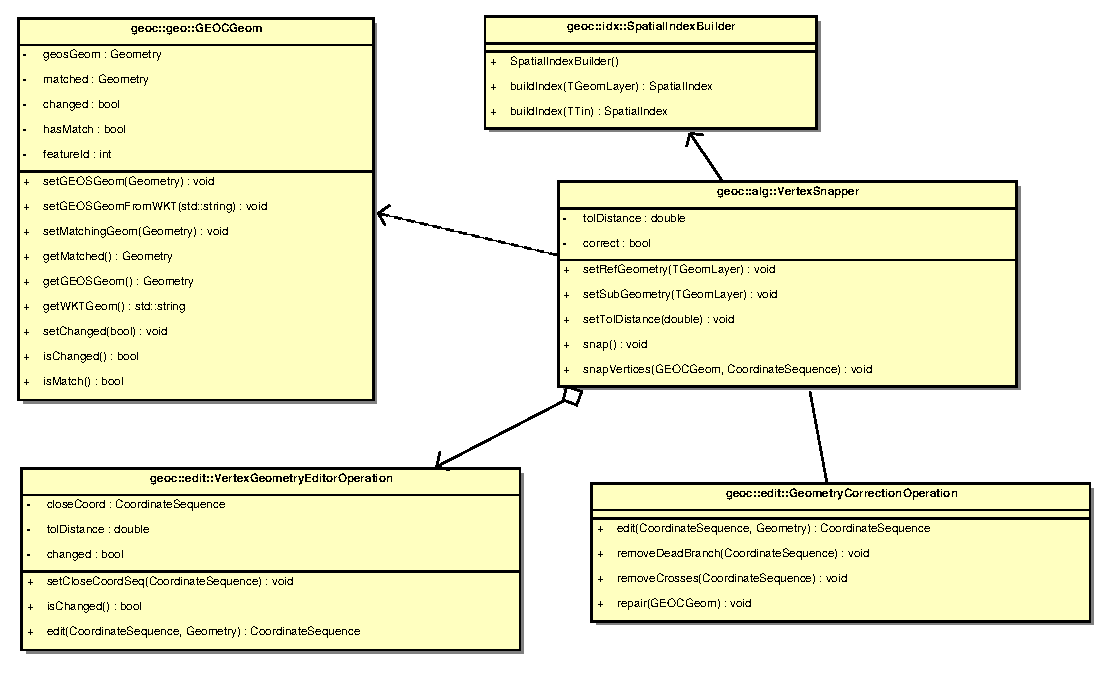
\includegraphics[width=420pt]{./pictures/uml-vs.pdf}
      \caption{UML diagram tříd pro VertexSnapper}
      \label{fig:uml-vs}
  \end{figure}

\vspace{2cm}
  \begin{figure}[t]
    \centering
      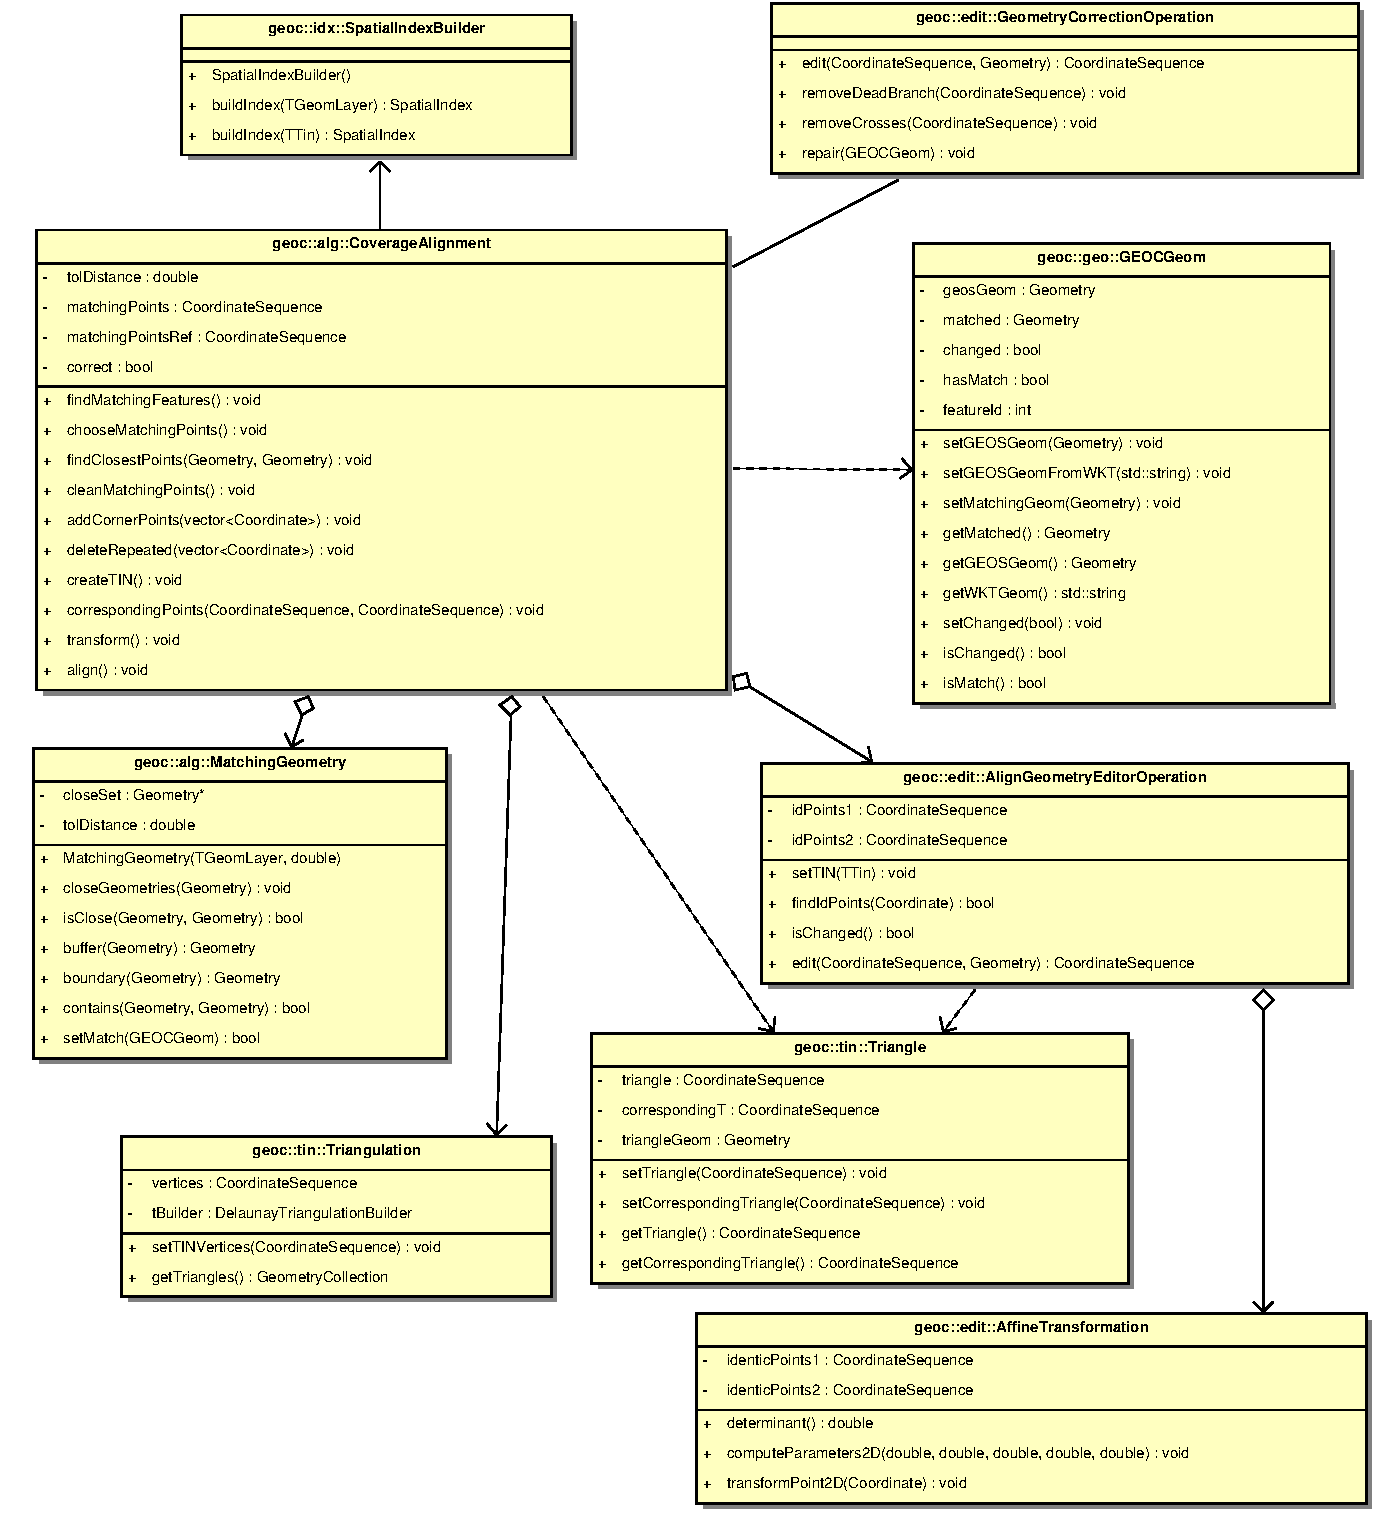
\includegraphics[width=420pt]{./pictures/uml-ca.pdf}
      \caption{UML diagram tříd pro CoverageAlignment}
      \label{fig:uml-ca}
  \end{figure}

\vspace{2cm}
  \begin{figure}[t]
    \centering
      \tiny
      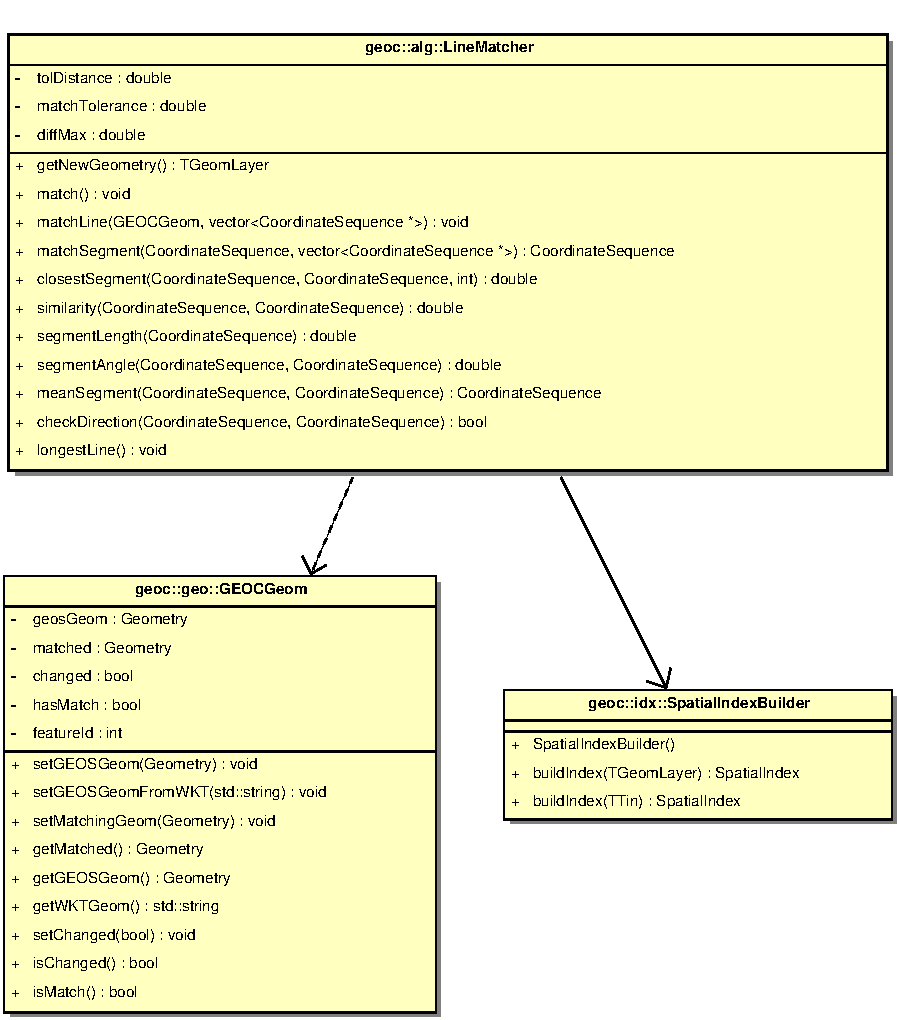
\includegraphics[width=420pt]{./pictures/uml-lm.pdf}
      \caption{UML diagram tříd pro LineMatcher}
      \label{fig:uml-lm}
  \end{figure}

%%%%%%%%%%%%%%%%%%%%%%%%%%%%%%%%%%%%%%%%%%%%%%%%%%%%%%%%%%%%%%%%%%%%%%%%%%%%%%%%%%%
%%                 PŘÍLOHA - UŽIVATELSKÁ PŘÍRUČKA                                %%
%%%%%%%%%%%%%%%%%%%%%%%%%%%%%%%%%%%%%%%%%%%%%%%%%%%%%%%%%%%%%%%%%%%%%%%%%%%%%%%%%%%
\chapter{Uživatelská příručka}
\label{priloha-prirucka}

Tato příručka je psána pro použití modulu \textbf{Conflate} v~Quantum GIS 1.9.0 , 
v~jiných verzích se může způsob načtení modulu, popř. i~jiné činnosti mírně lišit.

\section{Načtení zásuvného modulu}
\label{prirucka-nacteni}

Načtení zásuvného modulu lze provést ve~Správci zásuvných modulů.
\begin{center}
\textit{Zásuvné moduly~$\rightarrow$~Spravovat~zásuvné~moduly... 
(Plugins~$\rightarrow$~Plugin Manager...)}
\end{center}
Zde je třeba zaškrtnout \textit{Conflate Plugin}. Po~provedení tohoto kroku by se 
měla objevit ikonka modulu v~nástrojové liště a~také v~menu \textit{Zásuvné moduly}. 

  \begin{figure}[H]
    \centering
      
\includegraphics{./pictures/mActionConflate.pdf}
      \caption{Ikonka zásuvného modulu}
      \label{fig:ikonka}
  \end{figure}

Pokud se plugin nezobrazuje ve~Správci zásuvných modulů, je třeba nastavit cestu 
k~souboru~\textit{.so} v~\textit{Nastavení}.
\begin{center} 
\textit{Nastavení~$\rightarrow$~Volby~$\rightarrow$~Systém~$\rightarrow$~Cesty 
k~zásuvným modulům (Settings~$\rightarrow$~Options$\rightarrow$~System~$\rightarrow$
~Plugin paths)}
\end{center}


\section{Spuštění a nastavení dialogu}
\label{prirucka-spusteni}

\subsection{Výběr vstupních vrstev}
Před spuštěním dialogu \textit{Conflate} je třeba mít v~aktuálním projektu 
načteny vrstvy, které chceme zpracovávat. Pokud přidáme vrstvu až po~otevření
dialogu, lze ji načíst do~výběru vrstev tlačítkem \textit{Refresh}.
Po~otevření dialogu je třeba provést výběr \textbf{re\-ferenční vrstvy} 
(\textit{Reference Layer}) a~\textbf{upravované vrstvy} (\textit{Subject Layer}). 
Re\-ferenční vrstva je obvykle ta s~vyšší přesností, která se nebude měnit. 
Upravovanou vrstvu naopak chceme zarovnat k~vrstvě referenční. 
Obě vrstvy by měly být stejného geometrického typu (polygon~-~polygon, 
linie~-~linie, bod~-~bod).

\subsection{Metoda zpracování}
Dalším krokem je volba způsobu zpracování (\textit{Select the way of conflation}). 
Na~výběr jsou tyto metody, jejichž princip je naznačen na~obrázku \ref{fig:algorithms}.

\begin{itemize}
 \item \textbf{Přichycení vrcholů} (\textit{Snap Vertices}) - tato metoda vyhledá 
	blízké vrcholy z~obou datasetů a~změní polohu bodů upravované vrstvy tak, 
	aby odpovídala poloze blízkých bodů vrstvy referenční.
 \item \textbf{Zarovnání vrstev} (\textit{Coverage Alignment}) - princip této 
	metody je složitější. Na~rozdíl od~předchozí metody nepracuje s~jednotlivými
	body, ale s celými prvky. Upravuje i~ně\-které prvky, k nimž neexistují 
	žádné odpovídající ve~vrstvě refe\-renční, a~to na~základě změny okolních 
	prvků. Je proto vhodnější zejména pro datasety, které mají rozdílný počet
	prvků. Obecně je možné s~touto metodou dosáhnout přesnějších a~často
	reálnějších výsledků, avšak na~úkor času zpraco\-vání.
 \item \textbf{Napasování linií} (\textit{Match lines}) - tato metoda vyhledá
	odpovídající si úseky linií ze dvou různých vrstev. Takto nalezené
	páry zprůměruje a~vytvoří z~nich nové linie. Při volbě tohoto způsobu
	zpracování nezáleží na~tom, která vrstva je referenční a~která upravovaná.
	Napasování linií lze použít pouze na~dvojice liniových vrstev.
\end{itemize}

  \begin{figure}[H]
    \centering
      \def\svgwidth{400pt}
      \input{./pictures/algorithms.pdf_tex}
      \caption{Princip jednotlivých algoritmů}
      \label{fig:algorithms}
  \end{figure}

\subsection{Další nastavení}
Poté je třeba nastavit \textbf{toleranční vzdálenost} (\textit{Distance 
Tolerance}) v~jednotkách projektu. Tato vzdálenost udává, v~jaké maximální 
vzdálenosti mohou být odpovídající si prvky z~obou vrstev, a~jak moc se 
tedy může cílová vrstva měnit. V~ideálním případě by tato vzdálenost 
neměla přesahovat nejkratší segment geometrie všech prvků upravované vrstvy 
(tzn. nejkratší úsek linie nebo nejkratší stranu polygonu). Nevhodná volba této 
vzdálenosti může vést ke~vzniku nevalidních geometrií či nereálným výsledkům.

U~poslední metody (\textit{Match Lines}) se zviditelní ještě možnost nastavení
\textbf{kritéria podobnosti} \textit{Matching criterium}. Jedná se o~minimální 
podobnost dvou segmentů, která musí být dodržena pro jejich spárování. 
Tato hodnota se udává v~procentech. Při zadání $100 \%$ jsou výsledkem pouze 
naprosto totožné segmenty. Kritérium podobnosti se počítá na základě úhlu mezi 
segmenty, vzdálenosti jejich koncových bodů a~rozdílu jejich délek. 

Volba toleranční vzdálenosti a~metody zarovnání může výrazně ovlivnit rychlost 
zpracování, je proto doporučeno volit raději vždy menší vzdálenost a~jednodušší
metodu a~teprve po zobrazení výsledků případně parametry změnit.

Poslední nastavovanou možností je \textbf{automatická oprava geometrie}
 zaškrtnutím \textit{Try to repair invalid geometries}. Při této volbě se 
program pokusí opravit nově vzniklé nevalidní geometrie. Opravováno je pouze 
křížení úseků v~polygonu a~tzv. \uv{slepé větve}. Automa\-tická oprava  
může ovlivnit přesnost výsledku a~někdy i~vytvořit topologické chyby, proto 
je třeba ji používat opatrně. Při volbě \textit{Match Lines} není tato možnost
dostupná, jelikož uvedené situace nejsou u~liniových geometrií považovány
za~chybné.

\subsection{Výstupní vrstva}

Před spuštěním zpracování lze ještě nastavit název a~cestu, kam se má uložit
vý\-sledný soubor. Upravená vrstva se vždy uloží jako nová vrstva ve~formátu 
\textit{shapefile}. Do~pole \textit{Output shapefile} lze zadat \textbf{cestu 
k~výstupnímu souboru}, popřípadě ji vybrat pomocí tlačítka \textit{Browse} 
(\textit{Procházet}) vpravo. 

Pokud zadáte pouze název výstupní vrstvy nebo toto pole necháte prázdné, 
uloží se nová vrstva do~aktuálního adresáře pod daným názvem nebo pod názvem
upravované vrstvy s~příslušným pořadovým číslem. 

Po~nastavení všech parametrů se stisknutím tlačítka \textit{Process} 
spustí zpracování. 

\section{Výsledek}
\label{prirucka-vysledek}

Upravená vrstva se automaticky přidá do~otevřeného projektu v~QGISu.

V~dialogu zásuvného modulu se do~textového pole vlevo vypíše protokol o~zpracování.
Formát protokolu je popsán na~obrázku \ref{fig:protokol}.  

  \begin{figure}[ht]
    \centering
      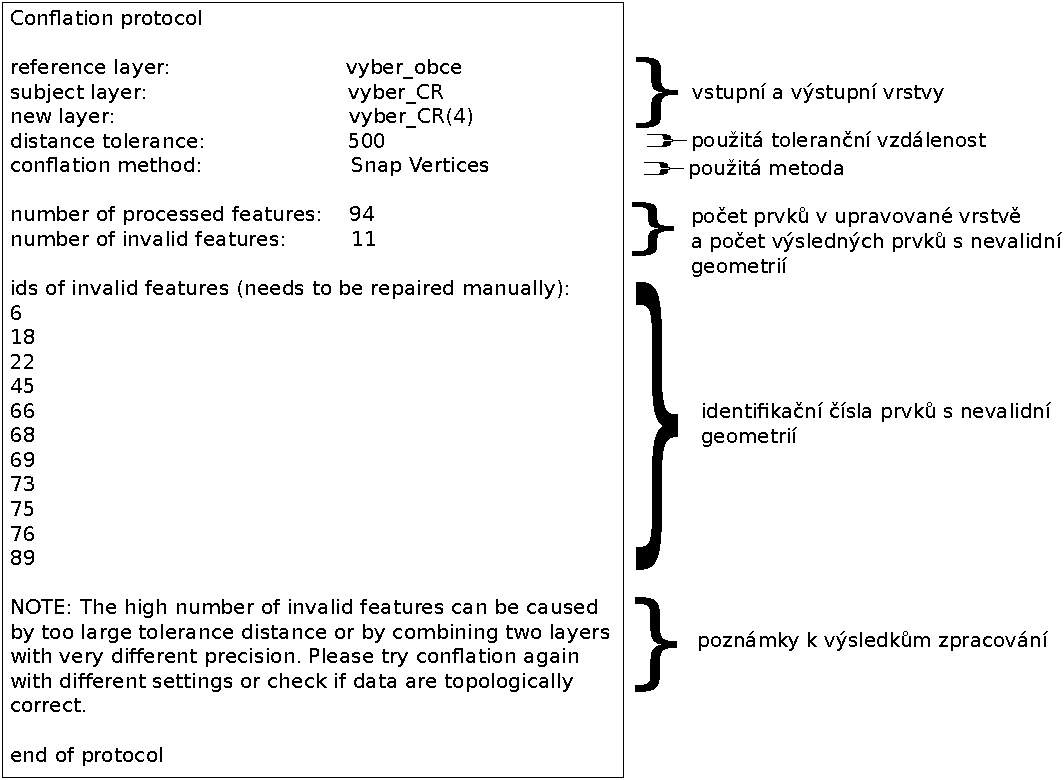
\includegraphics[width=420pt]{./pictures/protokol.pdf}
      \caption{Formát protokolu}
      \label{fig:protokol}
  \end{figure} 

Výsledkem zpracování mohou být i~nevalidní geometrie, jejichž identifikátory lze
nalézt v~protokolu. Proto jsou často nezbytné ještě závěrečné úpravy s~využitím
editačních nástrojů QGISu.


%%%%%%%%%%%%%%%%%%%%%%%%%%%%%%%%%%%%%%%%%%%%%%%%%%%%%%%%%%%%%%%%%%%%%%%%%%%%%%%%%%%
%%                 PŘÍLOHA - SCREENSHOTY                                         %%
%%%%%%%%%%%%%%%%%%%%%%%%%%%%%%%%%%%%%%%%%%%%%%%%%%%%%%%%%%%%%%%%%%%%%%%%%%%%%%%%%%%
\chapter{Screenshoty zásuvného modulu}
\label{priloha-screenshoty}

  \begin{figure}[H]
    \centering
      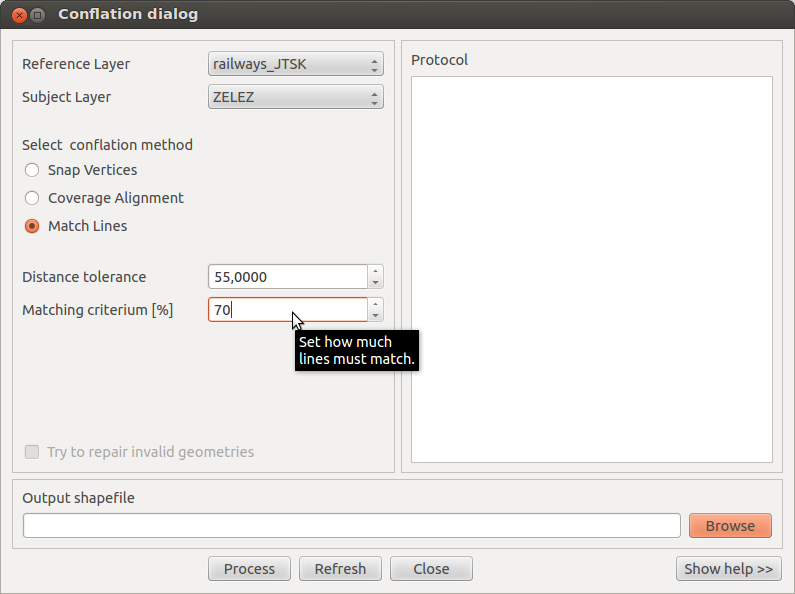
\includegraphics[width=360pt]{./pictures/dialog1.png}
      \caption{Dialog zásuvného modulu - nastavení}
      \label{fig:d1}
  \end{figure} 

  \begin{figure}[H]
    \centering
      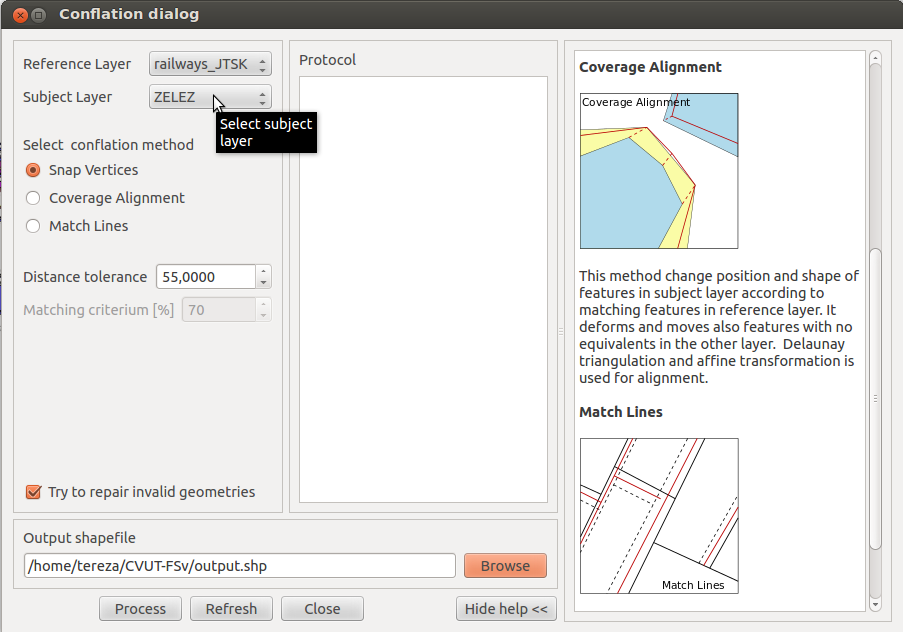
\includegraphics[width=360pt]{./pictures/dialog2.png}
      \caption{Dialog zásuvného modulu - nápověda}
      \label{fig:d2}
  \end{figure} 

  \begin{figure}[H]
    \centering
      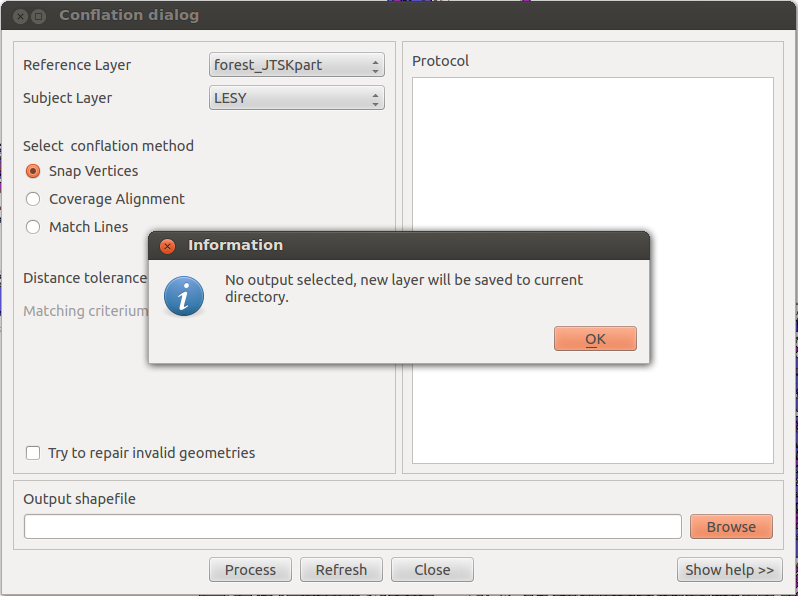
\includegraphics[width=360pt]{./pictures/dialog3.png}
      \caption{Dialog zásuvného modulu - upozornění}
      \label{fig:d3}
  \end{figure} 

  \begin{figure}[H]
    \centering
      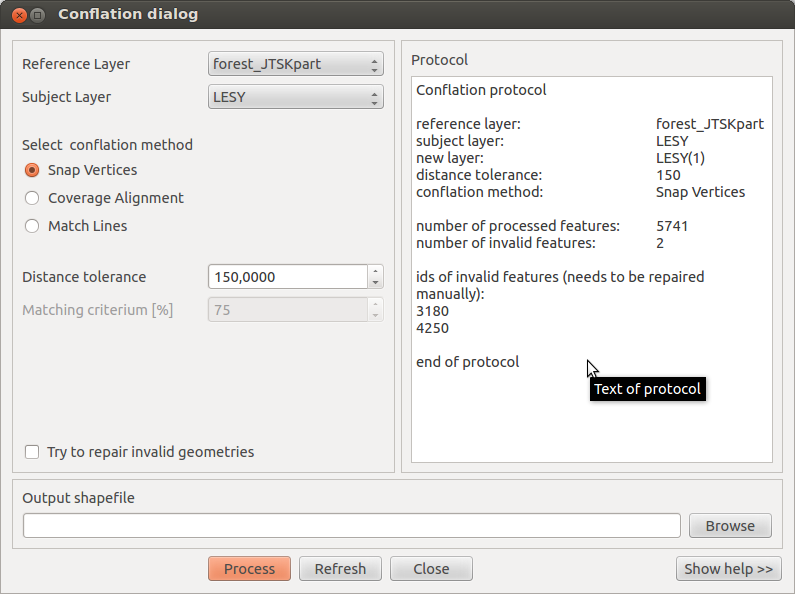
\includegraphics[width=360pt]{./pictures/dialog4.png}
      \caption{Dialog zásuvného modulu - protokol}
      \label{fig:d4}
  \end{figure} 

%%%%%%%%%%%%%%%%%%%%%%%%%%%%%%%%%%%%%%%%%%%%%%%%%%%%%%%%%%%%%%%%%%%%%%%%%%%%%%%%%%%
%%                 PŘÍLOHA - UKÁZKY                                              %%
%%%%%%%%%%%%%%%%%%%%%%%%%%%%%%%%%%%%%%%%%%%%%%%%%%%%%%%%%%%%%%%%%%%%%%%%%%%%%%%%%%%
\chapter{Ukázky zpracování dat}
\label{priloha-ukazky}

\section{VertexSnapper}
\label{ukazky-vs}

  \begin{figure}[H]
    \centering
      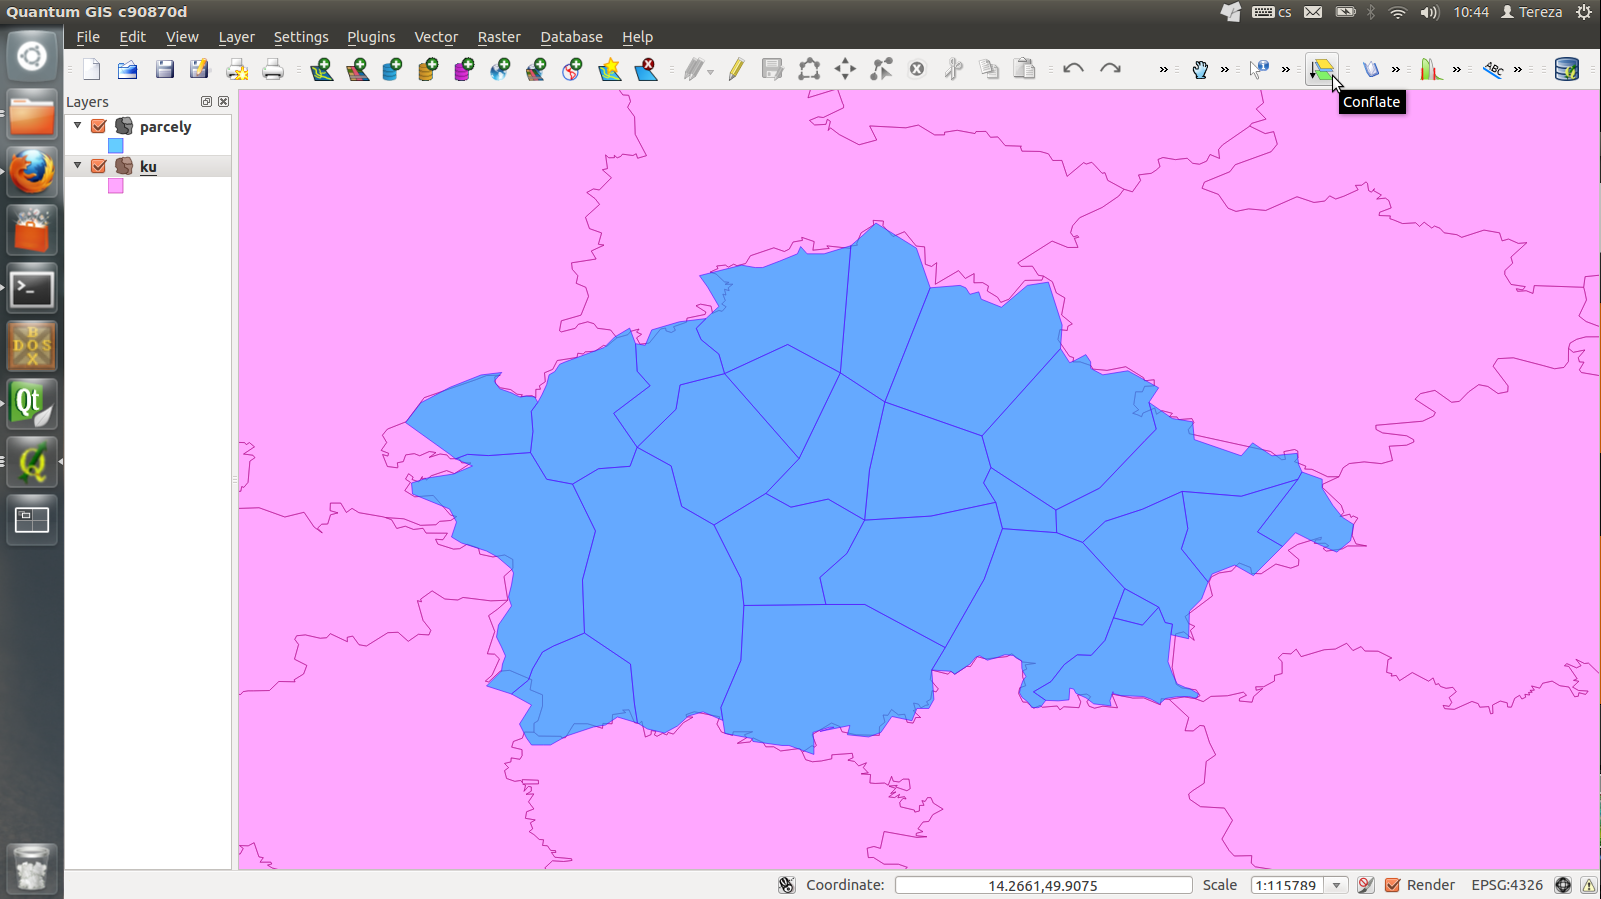
\includegraphics[width=400pt]{./pictures/test-vs1.png}
      \caption{VertexSnapper - vstupní data}
      \label{fig:vs1}
  \end{figure}

  \begin{figure}[H]
    \centering
      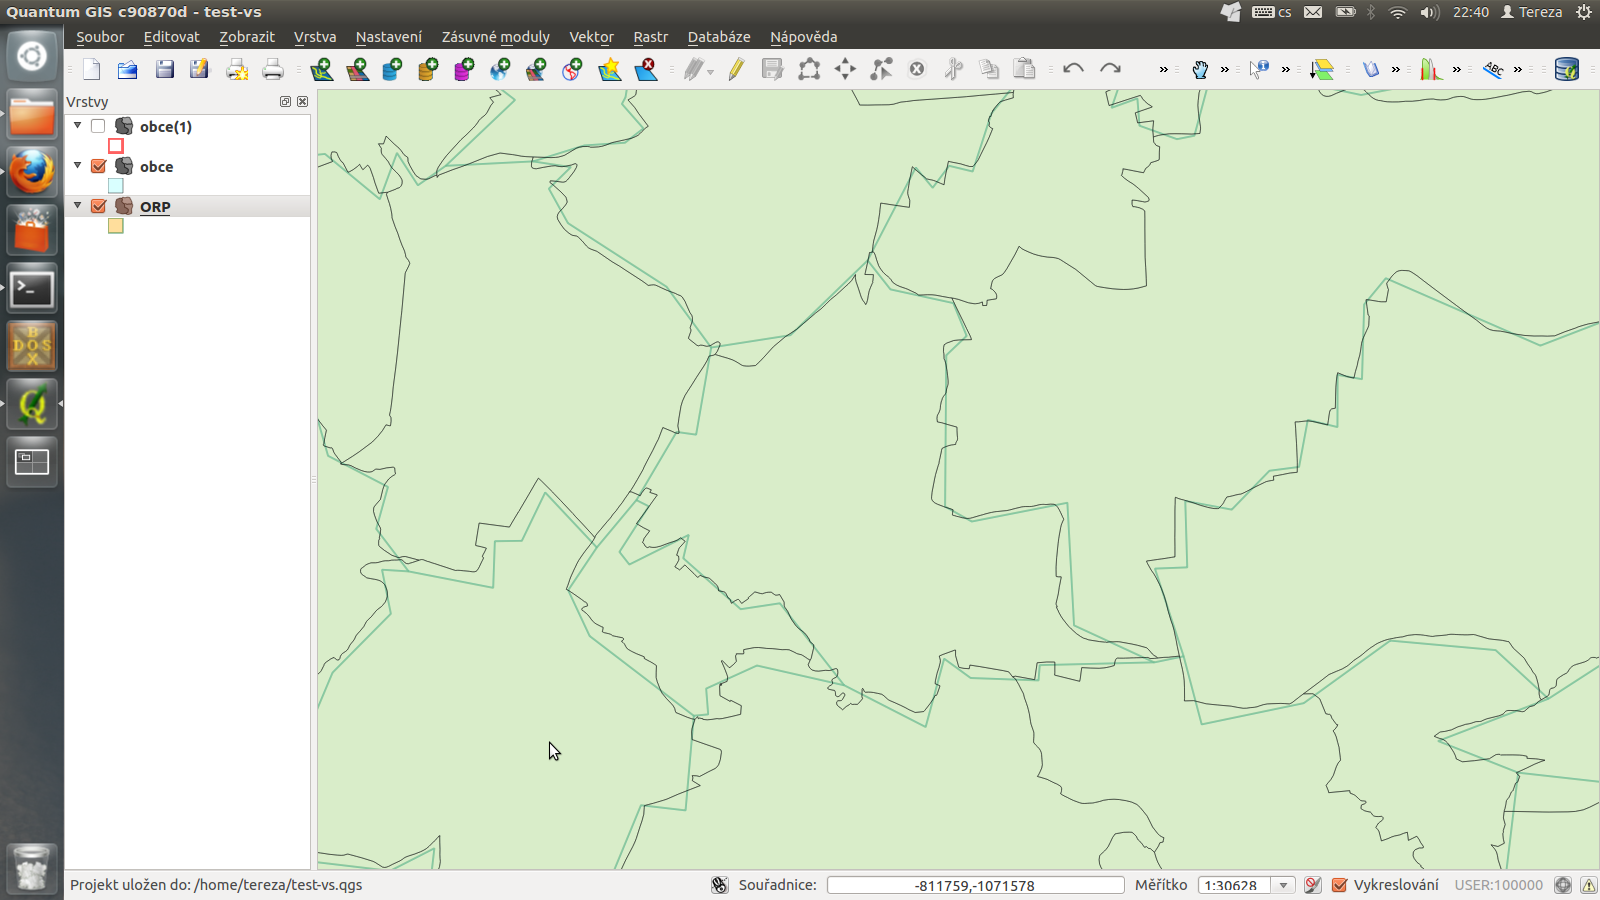
\includegraphics[width=400pt]{./pictures/test-vs2.png}
      \caption{VertexSnapper - výsledek zpracování}
      \label{fig:vs2}
  \end{figure}

  \begin{figure}[H]
    \centering
      \def\svgwidth{420pt}
      \input{./pictures/vs-porovnani.pdf_tex}
      \caption{VertexSnapper - porovnání}
      \label{fig:vs3}
  \end{figure}

\section{CoverageAlignment}
\label{ukazky-ca}

  \begin{figure}[H]
    \centering
      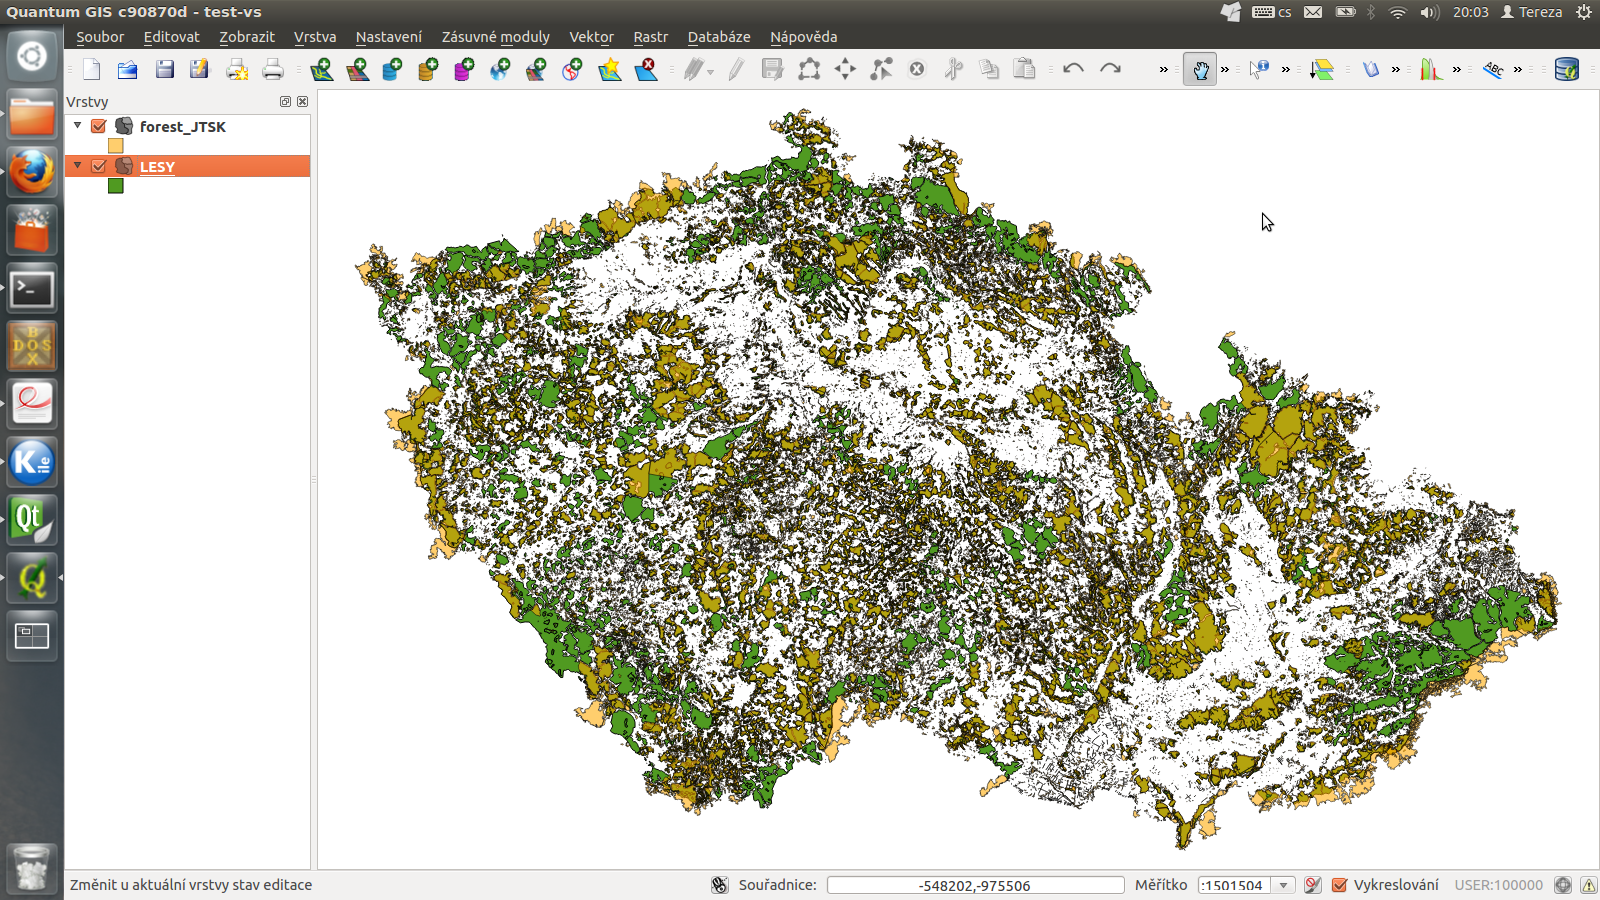
\includegraphics[width=400pt]{./pictures/test-ca1.png}
      \caption{CoverageAlignment - vstupní data}
      \label{fig:ca1}
  \end{figure}

  \begin{figure}[H]
    \centering
      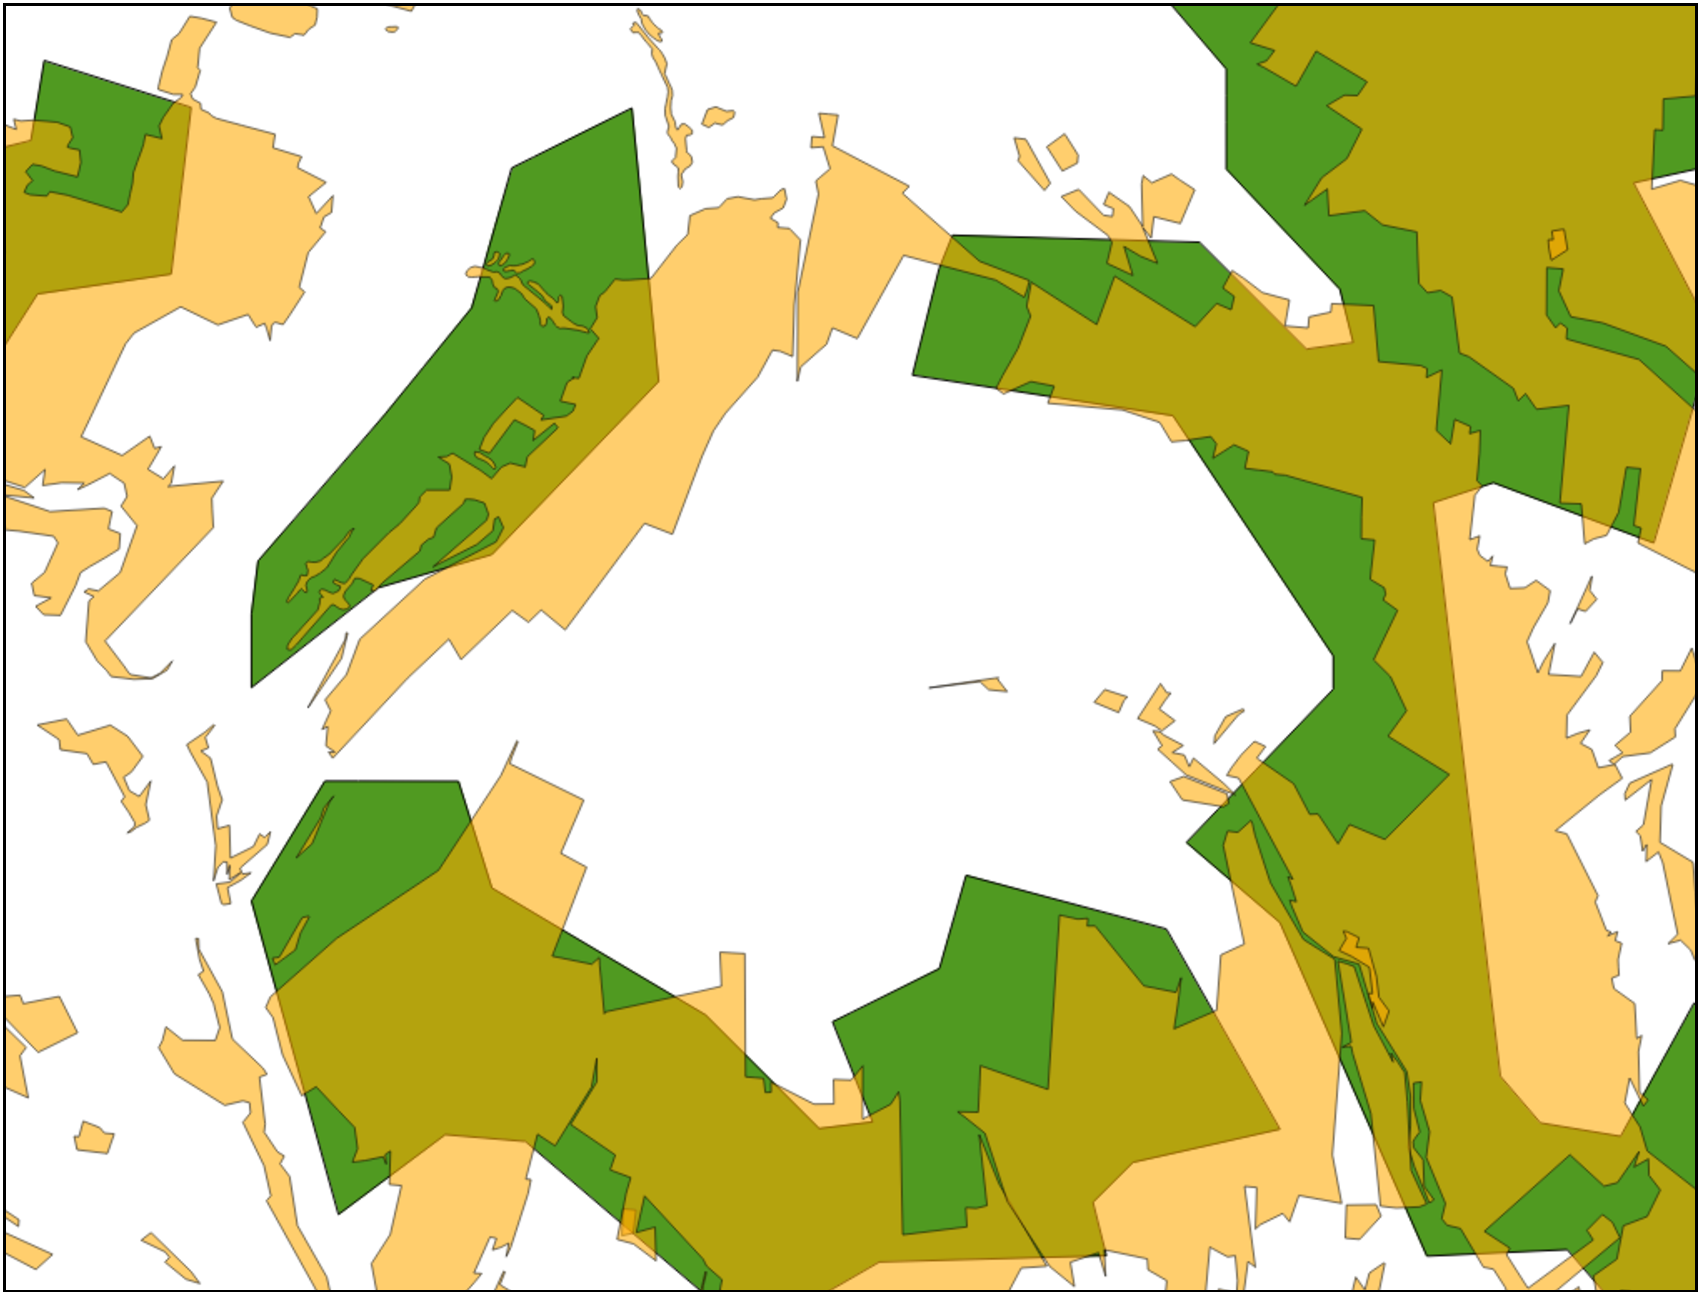
\includegraphics[width=360pt]{./pictures/test-ca2.pdf}
      \caption{CoverageAlignment - před zarovnáním}
      \label{fig:ca2}
  \end{figure}

  \begin{figure}[H]
    \centering
      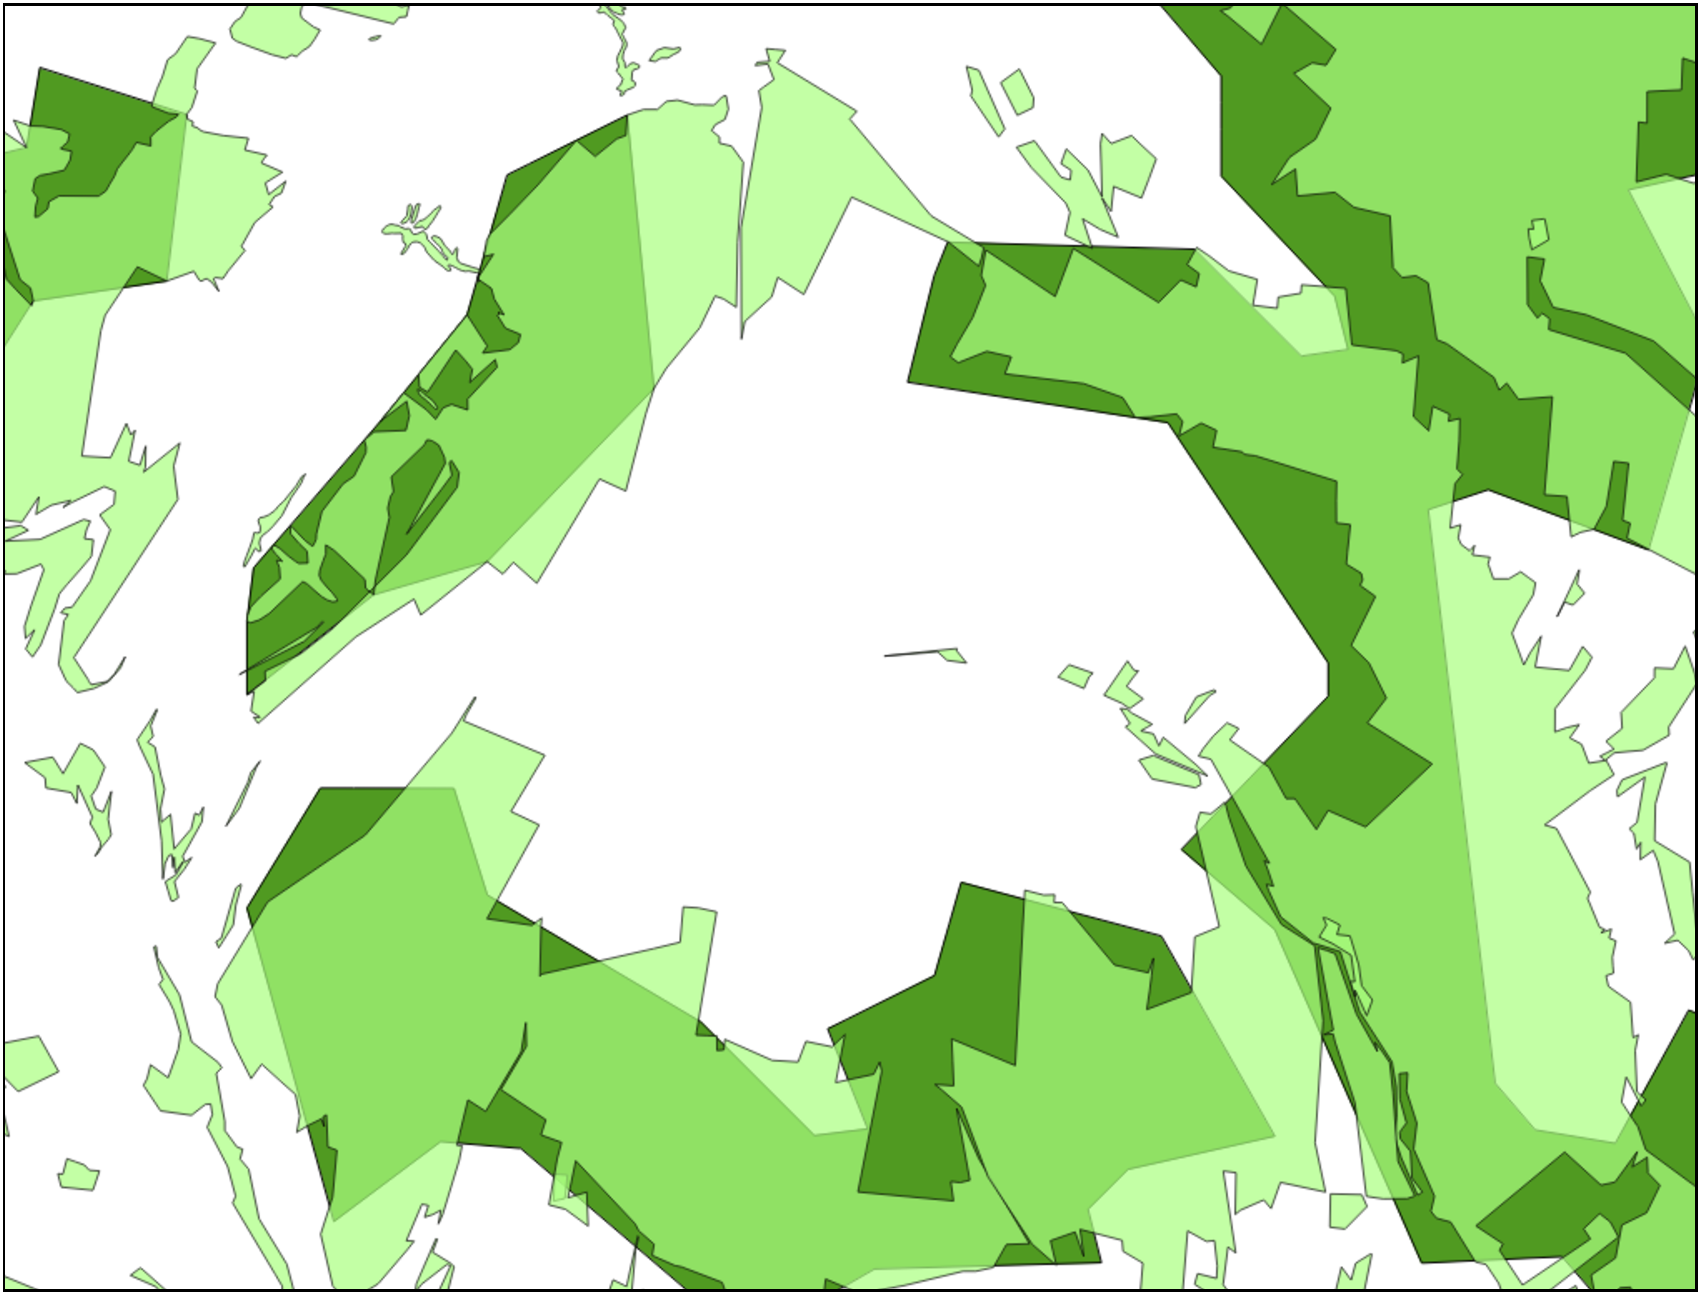
\includegraphics[width=360pt]{./pictures/test-ca3.pdf}
      \caption{CoverageAlignment - po zarovnání}
      \label{fig:ca3}
  \end{figure}

  \begin{figure}[H]
    \centering
      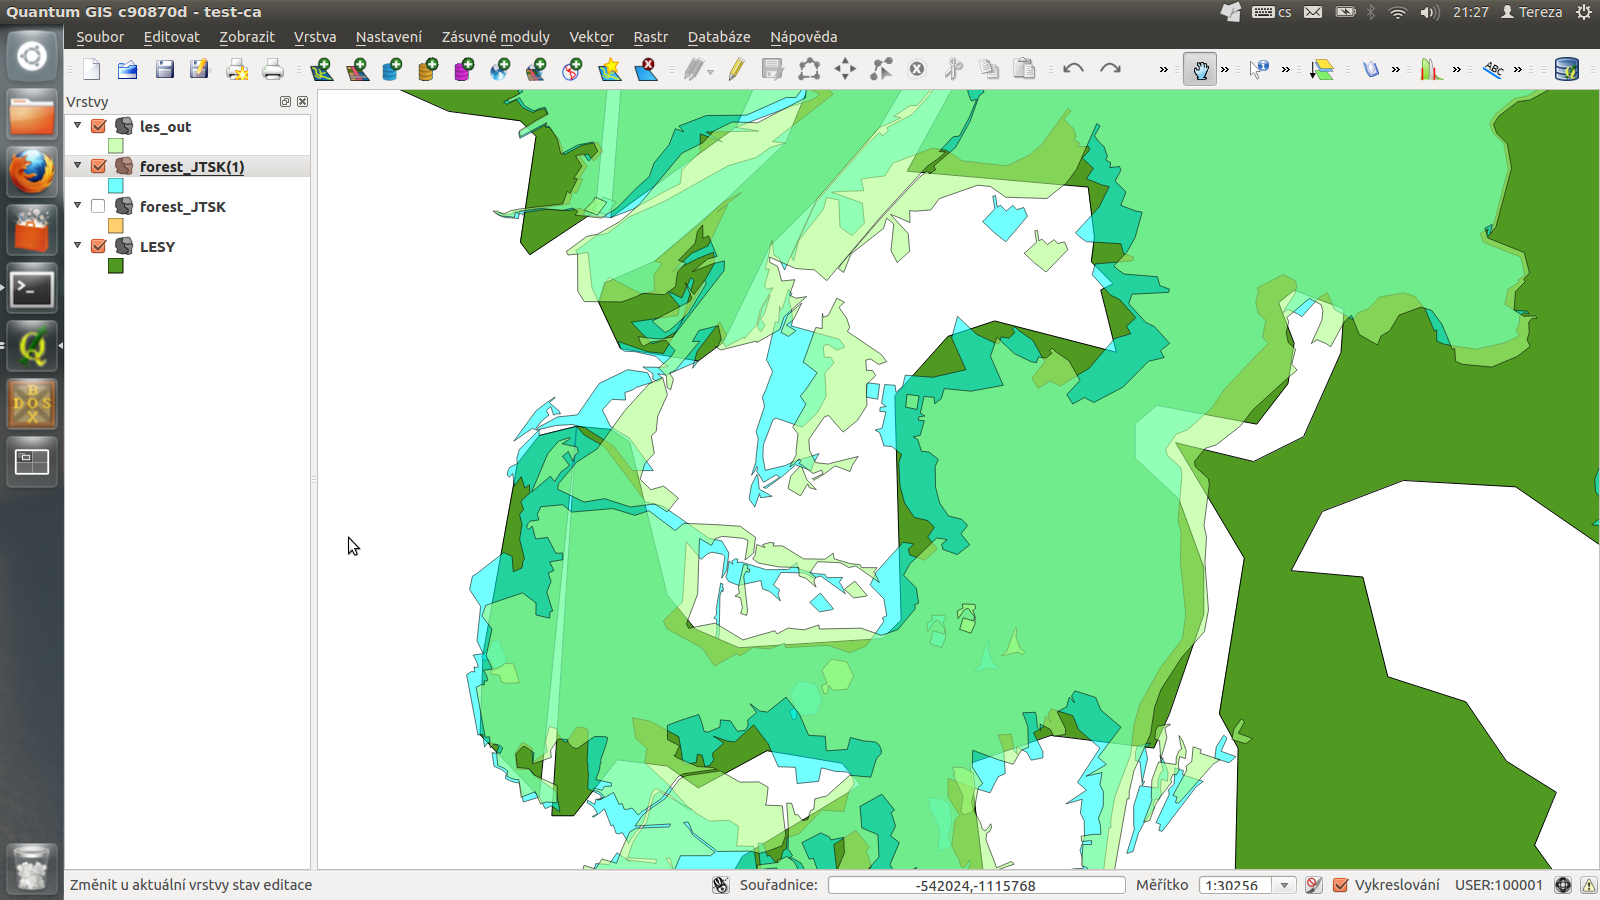
\includegraphics[width=400pt]{./pictures/test-ca4.png}
      \caption[CoverageAlignment- porovnání]{CoverageAlignment 
	- porovnání zarovnání s~toleranční vzdáleností 600~m~(zelená)
	a~1100 m (modrá)}
      \label{fig:ca4}
  \end{figure}

\section{LineMatcher}
\label{ukazky-lm}

  \begin{figure}[H]
    \centering
      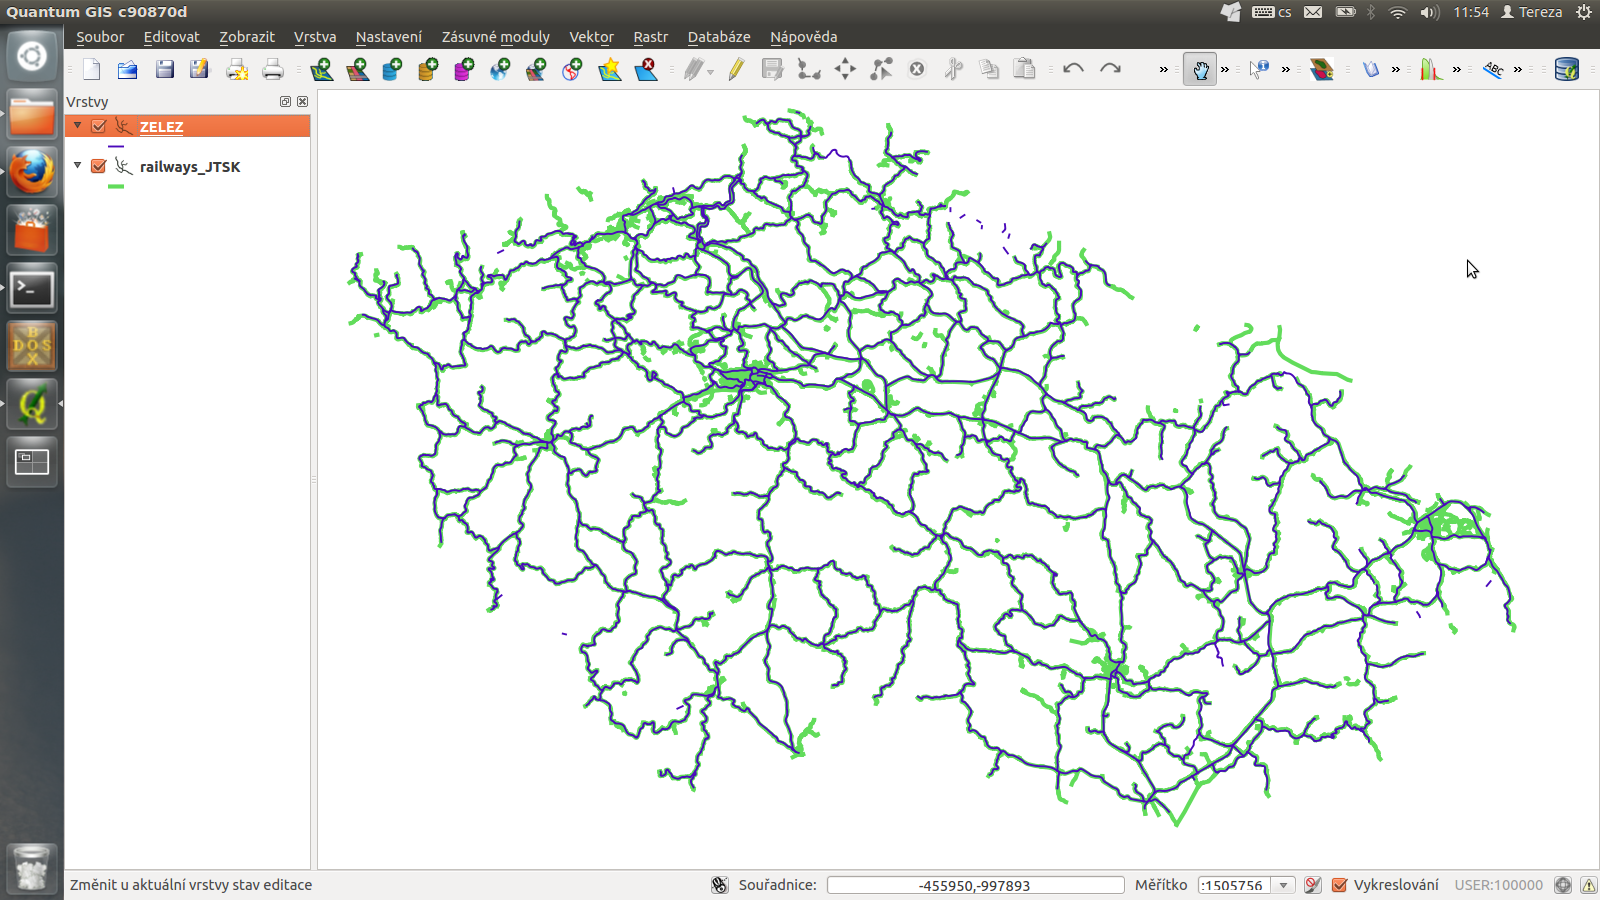
\includegraphics[width=400pt]{./pictures/test-lm1.png}
      \caption{LineMatcher - vstupní data}
      \label{fig:lm1}
  \end{figure}

  \begin{figure}[H]
    \centering
      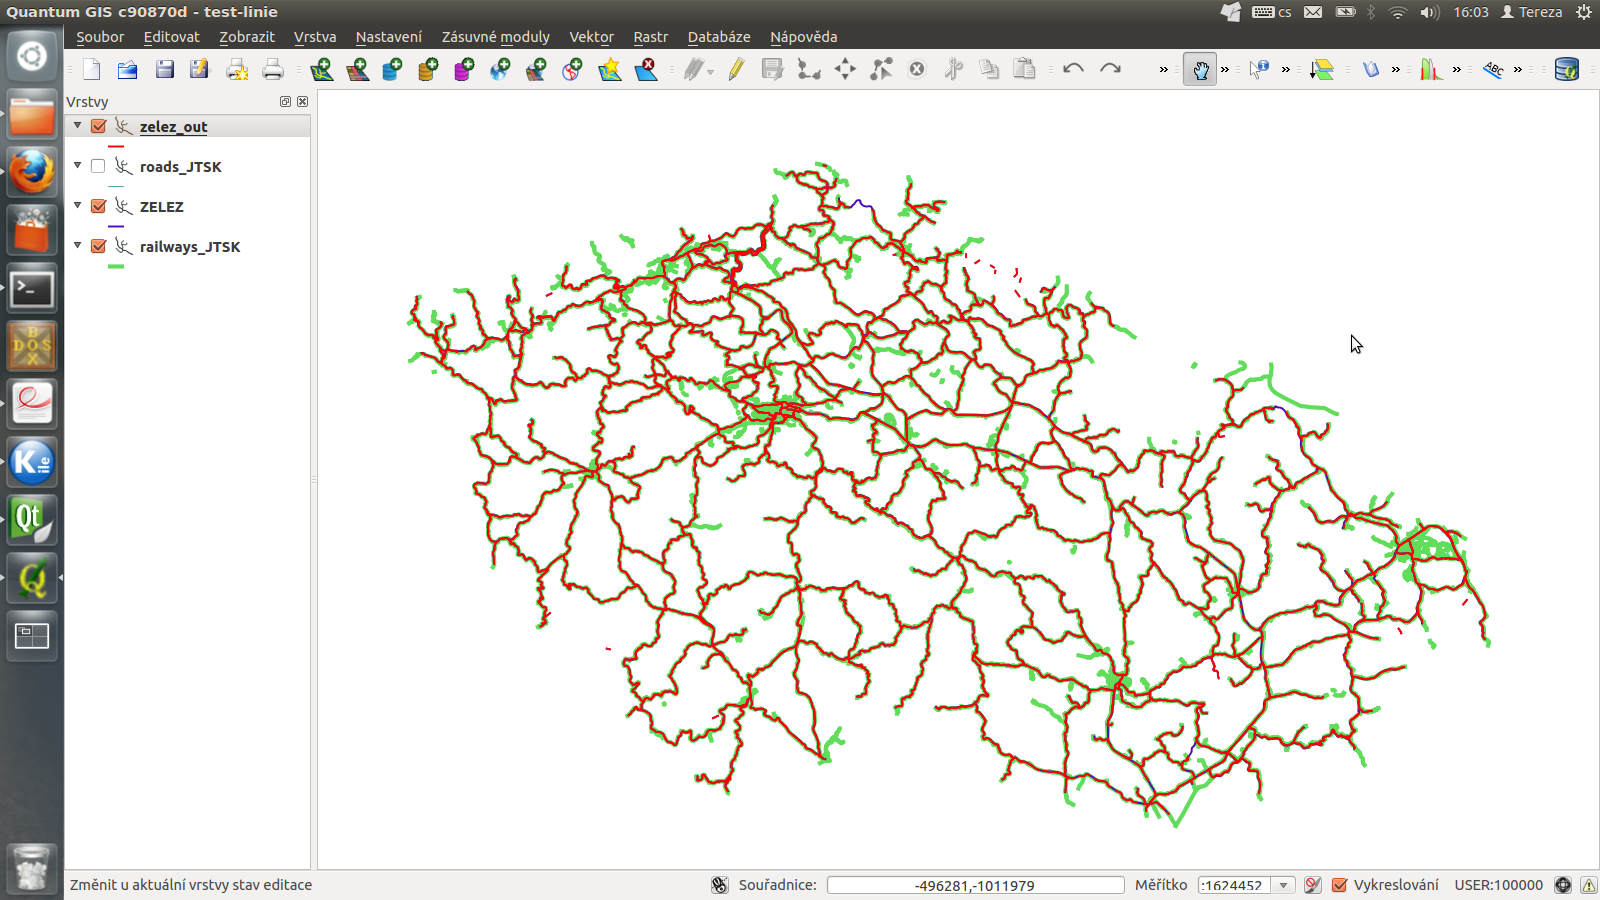
\includegraphics[width=400pt]{./pictures/test-lm2.png}
      \caption{LineMatcher - výsledek}
      \label{fig:lm2}
  \end{figure}  

  \begin{figure}[H]
    \centering
      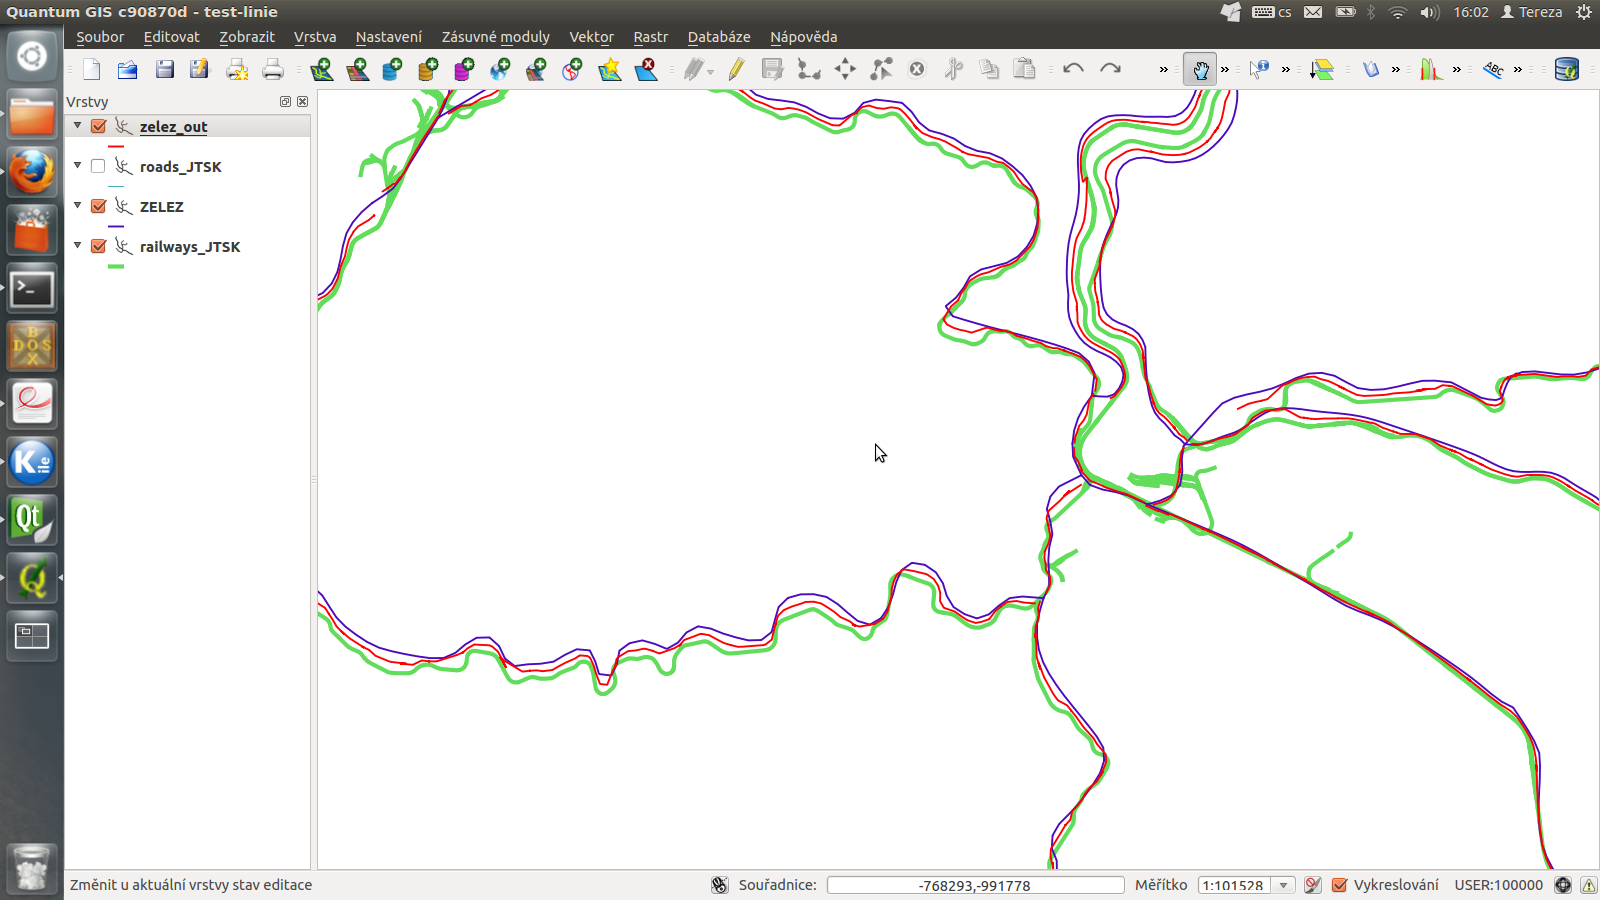
\includegraphics[width=400pt]{./pictures/test-lm3.png}
      \caption{LineMatcher - detail}
      \label{fig:lm3}
  \end{figure}  

%%%%%%%%%%%%%%%%%%%%%%%%%%%%%%%%%%%%%%%%%%%%%%%%%%%%%%%%%%%%%%%%%%%%%%%%%%%%%%%%%%%
%%                 PŘÍLOHA - OBSAH CD                                            %%
%%%%%%%%%%%%%%%%%%%%%%%%%%%%%%%%%%%%%%%%%%%%%%%%%%%%%%%%%%%%%%%%%%%%%%%%%%%%%%%%%%%
\chapter{Obsah CD}
\label{priloha-obsahCD}

\setlength{\unitlength}{.5mm}
\begin{picture}(250, 220)
  \put(  0, 212){\textbf{.}}
  \put(  1, 200){\line(0, 1){5}}
  \put(  1, 200){\line(1, 0){10} {\textbf{ conflate}}}
  \put( 16, 190){\line(0, 1){8}}
  \put( 16, 190){\line(1, 0){10} {\textbf{ src}}}
  \put(150, 190){ zdrojové soubory pluginu}
  \put( 16, 180){\line(0, 1){10}}
  \put( 16, 180){\line(1, 0){10} {\textbf{ doc}}}
  \put(150, 180){ dokumentace vygenerovaná pomocí doxygen}
  \put( 16, 170){\line(0, 1){10}}
  \put( 16, 170){\line(1, 0){10} { readme.txt}}
  \put(150, 170){ návod a základní informace}
  \put( 16, 160){\line(0, 1){10}}
  \put( 16, 160){\line(1, 0){10} { libqgsconflate.so.1.0.0}}
  \put(150, 160){ přeložená aplikace}
  \put(  1, 150){\line(0, 1){60}}
  \put(  1, 150){\line(1, 0){10} {\textbf{ geoc}}}
  \put( 16, 140){\line(0, 1){8}}
  \put( 16, 140){\line(1, 0){10} {\textbf{ src}}}
  \put(150, 140){ zdrojové kódy knihovny}
  \put( 16, 130){\line(0, 1){10}}
  \put( 16, 130){\line(1, 0){10} {\textbf{ doc}}}
  \put(150, 130){ dokumentace vygenerovaná pomocí doxygen}
  \put( 16, 120){\line(0, 1){10}}
  \put( 16, 120){\line(1, 0){10} { readme.txt}}
  \put(150, 120){ návod a základní informace}
  \put( 16, 110){\line(0, 1){10}}
  \put( 16, 110){\line(1, 0){10} { libgeoc.so.1.0.0}}
  \put(150, 110){ přeložená knihovna}
  \put(  1, 100){\line(0, 1){50}}
  \put(  1, 100){\line(1, 0){10} {\textbf{ testing}}}
  \put( 16,  90){\line(0, 1){8}}
  \put( 16,  90){\line(1, 0){10} {\textbf{ src}}}
  \put(150,  90){ zdrojové soubory testovací aplikace}
  \put( 16,  80){\line(0, 1){10}}
  \put( 16,  80){\line(1, 0){10} {\textbf{ sample\_data}}}
  \put(150,  80){ testovací data}
  \put( 16,  70){\line(0, 1){10}}
  \put( 16,  70){\line(1, 0){10} { readme.txt}}
  \put(150,  70){ návod a základní informace}
  \put( 16,  60){\line(0, 1){10}}
  \put( 16,  60){\line(1, 0){10} { geoc\_testing}}
  \put(150,  60){ testovací aplikace}
  \put( 16,  50){\line(0, 1){10}}
  \put( 16,  50){\line(1, 0){10} { testing.sh}}
  \put(150,  50){ bash skript pro testování}
  \put(  1,  40){\line(0, 1){60}}
  \put(  1,  40){\line(1, 0){10} {\textbf{ text}}}
  \put( 16,  30){\line(0, 1){8}}
  \put( 16,  30){\line(1, 0){10} {\textbf{ latex}}}
  \put(150,  30){ zdrojové soubory textu této práce}
  \put( 16,  20){\line(0, 1){10}}
  \put( 16,  20){\line(1, 0){10} { tereza-fiedlerova-bp-2013.xls}}
  \put(150,  20){ anotace práce}
  \put( 16,  10){\line(0, 1){10}}
  \put( 16,  10){\line(1, 0){10} { tereza-fiedlerova-bp-2013.pdf}}
  \put(150,  10){ tento text}
  \put( 16,   0){\line(0, 1){10}}
  \put( 16,   0){\line(1, 0){10} { zadani-oficialni.jpeg}}
  \put(150,   0){ naskenované oficiální zadání práce}
\end{picture}
